\chapter{Introdution}
Every business has its own objectives, processes, and requirements. Above all, today’s 
businesses need technologies with complete functions which can bridge the gap between business 
processes and people. To run a large organization with multiple departments and teams successfully, 
an ERP system gives a helping hand by synchronizing all information and communication within the organization. 
ERP is a combination of software and company’s activities performed to manage operations. With ERP software, 
the entire project value chain is aligned and critical processes are streamlined effectively. \newline \newline
Under an unmanaged system, various business processes within an organization utilize multiple disparate 
applications to manage similar operations. This leads to chaotic data transfer, time-consuming processes, and 
security gaps due to lack of access control. \newline \newline
For many small and midsize businesses (SMBs), it’s not a matter of if they will need enterprise resource 
planning (ERP) software, it’s a matter of when they will need it. As the company continues to grow, 
managing all that information across platforms becomes costly, time-consuming and prone to mismanagement. \newline \newline
Odds are good that a business relies on various software integrations to streamline data and access it cross-departmentally. 
But integrating multiple applications isn’t cheap. \newline \newline
Between license fees, staffing, training, operations and the labor required to get them to work well 
together (if they even work together at all), the price of owning and integrating multiple pieces of 
software can add up real fast. \newline \newline
So Enterprise resource planning (ERP) systems are used by organizations looking to manage 
their business functions within a centralized and integrated system. ERP is commonly used by 
companies working within the supply chain to help keep track of all the moving parts of manufacturing 
and distribution. However, ERP can be utilized by a number of different industries including those in 
healthcare, nonprofit groups and hospitality. Organizations needing to manage their 
staff, customers and inventory can all rely on ERP benefits.


%Some of the \textbf{greatest} 
%discoveries in \underline{science} 
%were made by \textbf{\textit{accident}}.


\chapter{ERP}
We now get the problem of integrated complex systems and how it will affect our business if not dealt with in the 
right manner, they need to be managed in an efficient way and handle the flow of data. We also introduced an 
ERP solution to solve this problem but what exactly is an ERP? and how will it help? \newline \newline
\textbf{ERP} stands for “Enterprise Resource Planning”	 
it’s a management software that integrates core business processes of a company by maintaining a common database. \newline \newline
A company usually consists of multiple departments and each department has its own functions 
processes that are performed within the region of this department but there exist the integrated 
business processes that companies use to perform their work which cut across the departments. 
ERP provides a way to manage these integrated processes from beginning to end by facilitating information 
sharing and connection between these departments. \newline \newline
ERP systems usually group common Function areas into so-called business Module like\\

\begin{adjustwidth}{2cm}{}
\textbf{Financial management} This module manages your capital inflow and outflow. It covers standard Accounting \& Finance transactions like ledger, balance sheet, tax management, and payments. The module also generates financial reports for different departments and business units.\\\\
\textbf{CRM} This module helps you to boost customer service and, eventually, profit. It manages leads, opportunities, and customer issues. Likewise, it provides a 360-degree profile of your customers by consolidating data like their social media activities, purchase history, and past interactions with support reps.\\\\
\textbf{Sales \& Marketing} This module handles sales workflows like sales inquiries, quotations, sales orders, and sales invoices. The Sales and CRM modules work together to speed up the sales cycle and earn the company more profits.\\\\
\textbf{Manufacturing} This module is sometimes referred to as Engineering or Production. It helps businesses make manufacturing more efficient in areas, such as product planning, materials sourcing, daily production monitoring, and product forecasting.\\\\
\end{adjustwidth}

ERP job is to coordinate between the various systems that the business needs and make seamless integration with a shared database between them, hence eliminating common problems like

\begin{itemize}
    \item No real-time data access for other departments.
    \item Latency to get information.
    \item More than one department having a need for the same data will cause high cost as data maintenance will increase.
    \item Shared data will need to be synchronized or a department will think it’s lacking or having more than its needs.
    \item Moving information from one department to another is more prone to errors.
    \item Numerous disparate information systems are developed individually over time.
    \item Integrating date takes time and money.
    \item Inconsistency and Duplication of data.
    \item Lack of timely information leads to customer dissatisfaction and loss in revenue.
\end{itemize}

%\begin{figure}
%    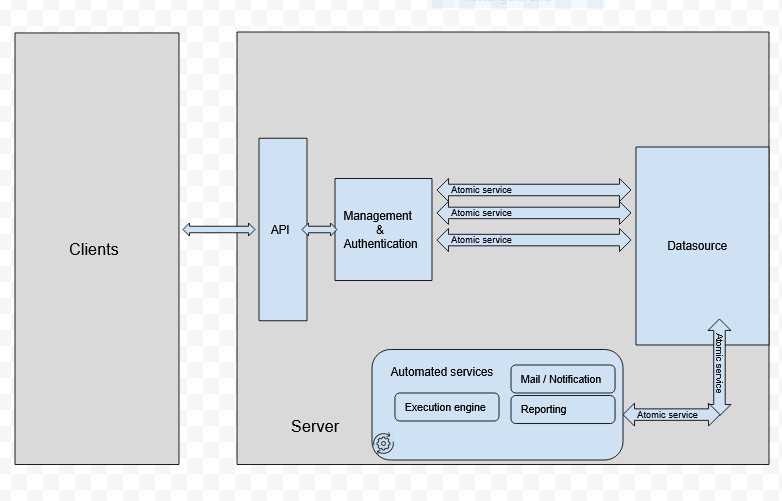
\includegraphics[width=\linewidth]{system_structure}
%    \caption{Test}
%    \label{fig:system_structure}
%\end{figure}


\chapter{The ERP}

The ERP is the name of our implementation of an ERP solution and using this name will always refer to our implementation.\\\\
The ERP has two main components
\begin{itemize}
    \item The main system which handles the system requests, controls the flow of data, and handles the users’ data.
    \item The system Modules that handle the business processes, We have a variety of modules to handle business needs.
\end{itemize}

\section{Main System}
Here we will talk about The ERP Features, Development, and internal structure and explore each component in the structure. Let’s begin with The features

\subsection{System Features}
The ERP is Open source, cross-platform, and cloud-based, so users can use it from homes, so no need for the companies using it to have huge buildings or offices to hold down their employees. This will help startups to push their businesses out without the need for huge financial support. Also, The ERP is multi-organizational, meaning that multiple organizations can use it at the same time. Finally, The ERP is very modular in design and can be expanded easily due to its modularity and simplicity.

\subsection{Development}
The ERP server and main functionality are written in C\# based on the brand new open source and cross-platform framework Asp.net core developed by Microsoft.\\\\
Modules services are written in C++ and compiled as DLL files and then gets loaded by the ERP when needed at runtime. Client-side is mostly written using Angular framework with some libraries like Bootstrap and JQuery. For Data storage we used Microsoft SQL server and MySQL database management systems and tools like swagger for API documentation. Next, you will find a table summarizing the tools used for development. Let’s talk a little bit about the main tools we use and why we chose them.
\\
\begin{adjustwidth}{2cm}{}
    \textbf{Asp.net core}
    \begin{adjustwidth}{1cm}{}
        Is a cross-platform, open-source, high-performance framework for building 
      Cloud-based, Internet-connected applications. With ASP.NET Core, you can
      \begin{itemize}
        \item Build web apps and services, IoT apps, and mobile backends
        \item Use your favorite development tools on Windows, macOS, and Linux
        \item Deploy to the cloud or on-premises
        \item Run on .Net Core or .Net Framework
      \end{itemize}
    \end{adjustwidth}
    \textbf{Why}
    \begin{adjustwidth}{1cm}{}
        Before we list the reasons, we’d like to point out that the main goal or reason
      is learning new stuff and get the work done by this stuff\\
      This framework is not mature enough and there is not that much of a community using it to help us when we face problems but we accepted the challenge and went on with it
      \\\\
      Here are some of the main reasons
      \begin{itemize}
        \item It’s a redesign of Asp.net 4.x with architectural changes that result in a leaner and more modular framework
        \item Open-source
        \item Cross-platform
        \item Easy integration of the client-side framework
        \item MVC easily implemented
        \item Built-in dependency injection
        \item A lightweight, high-performance, and modular HTTP request pipeline
        \item Ability to host on IIS, Nginx, Apache, Docker, or self-host in your own process (Kestrel)
      \end{itemize}
    \end{adjustwidth}
    \textbf{DLL}
    \begin{adjustwidth}{1cm}{}
        Stands for Dynamic Link Library and it’s a Shared Library that can be used by more than one program at the same time and can be loaded into the program while running.
By wrapping each of The Erp Modules services in a DLL file, we can modularize our software and load them when needed only, this will help us save a lot of resources and enable us to have the ability to sell each module, maintain them and apply repairs, or upgrade to them separately and the system functions will not be affected.
\\\\
    \end{adjustwidth}
\end{adjustwidth}


\subsection{Tools}

\begin{table}[h!]
\centering
\begin{tabular}{ |p{3cm}|p{3cm}|p{3cm}|p{3cm}|  }
    \hline
    \textbf{Tool} & \textbf{usage} & \textbf{Requirement} & \textbf{Programming language}\\
    \hline
    Asp.net core  & server and main functionality  & net core 2.2.x
    runtime
    Or SDK  & C\#\\
    \hline
    Angular  & Client-side development  & Node.js 8.12.0
    Angular CLI
    7.3.8  & Typescript
    Javascript
    Css
    Html\\
    \hline
    Entity framework
core  & An ORM to deal with the
database  & shipped with the
framework  & C\#\\
    \hline
    DLL & Contain modules and main
    system services  & C++ compiler  & C++\\
    \hline
    Microsoft SQL
server  & Data Source to store
system data  & Microsoft SQL
server  & SQL\\
    \hline
    MySql  & Data Source to store
    system data  & MySql  & SQL\\
    \hline
\end{tabular}
\caption{summary of the ERP tools used for development}
\label{table:1}
\end{table}


\subsection{System Structure}

The main components of the system are shown in the fugure \ref{fig:system_structure} which will be explored in
detail in the coming sections

\begin{figure}
    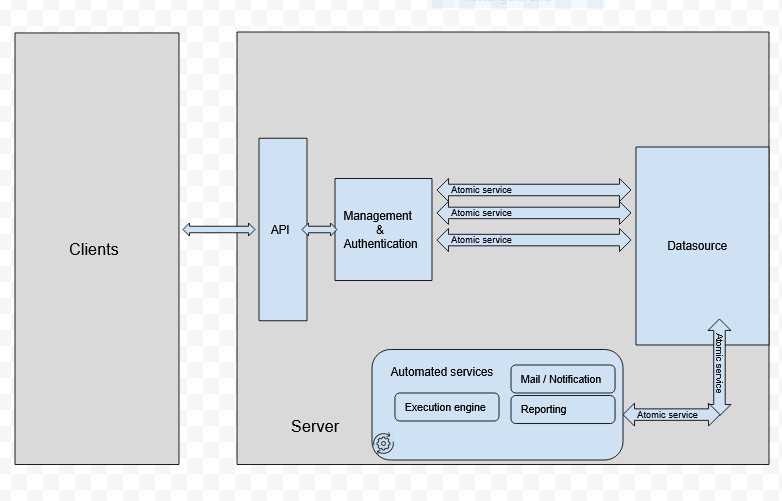
\includegraphics[scale=0.5, width=100mm]{system_structure}
    \centering
    \caption{ERP System Structure}
    \label{fig:system_structure}
\end{figure}


\subsubsection{System Main Components}

\begin{adjustwidth}{2cm}{}
    \textbf{API}
    \begin{adjustwidth}{1cm}{}
        Stands for Application Programming Interface, is an interface that simplifies the access to
one’s application services from another application, so it’s the gateway to The ERP
Services.\\\\
For web-based API as in The ERP, each service will have a URL like \url{http://www.TheErp.com/app/GetProducts }, and in order to use this service an HTTP request will
be sent to this URL with some data (if required by the services), then the service gets invoked,
and then return the result in the form of HTTP response.\\\\
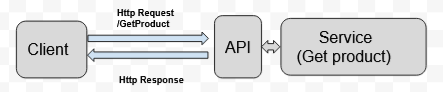
\includegraphics[width=100mm,scale=0.5]{system_api}\\\\
The ERP API is well documented using the swagger tool, so any external system that is
interested in using The Erp services can use this documentation.\\\\
    \end{adjustwidth}

    \textbf{Role Management \& Authentication}\\
    
    \begin{adjustwidth}{1cm}{}
        It is used to limit the access for certain services in The ERP.
        First, it Authenticates the incoming requests, in case of browser we use cookie
        Authentication; otherwise, Jwt Authentication is used, after authentication we can find out
        some info about the invoker like username, user id, roles (Administrator, manager, ..etc), and
        company name because like we said before, The ERP can be used by multiple organizations
        at the same time, so the company must be included. The reason why we can find this info, is
        after a login request from a client has been validated, this info gets encrypted as a cookie in
        case of a client browser or a token otherwise, and sent back with the HTTP response to the
        login request, so that when a client calls a service which requires Authentication, the client
        must include the cookie or the token it received after successfully logged it in the HTTP
        request and then it gets decrypted and the information can be deduced.\\\\
    \end{adjustwidth}

    \textbf{Services}\\
    
    \begin{adjustwidth}{1cm}{}
        First of all, let’s define the term service. A service, in the case of The ERP, is a job that we
want The ERP to do it for us, like getting an order, sending an email, or giving a report of the
financial situation ..etc.
If we look deeper into these jobs we can find out that some of them can be divided into
smaller jobs. For example, getting an order, it first checks that the products in the order are in
stock then accepts the payment, if they are, then send the order; otherwise, orders the
manufacturing to start to produce this product and inform the customer.
These smaller jobs are called, in our system, Atomic services because they can’t be divided
into smaller jobs.\\
These Atomic services can be used as a building block for other big services, such as in the
case of sending an order. And it can be used as a service itself. So the bottom line is that The
Erp is only containing services that are atomic in nature.
Above that, the services are a composite of these Atomic services.\\\\
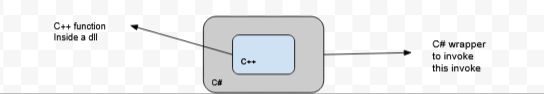
\includegraphics[width=100mm,scale=0.5]{atomic_service}\\\\
If we zoom in on atomic services we will find out that they consist of C++ functions and C\#
wrapper to serve as an interface to the C++ code.\\
Another kind of the services The ERP provides is the Automated Services .
Automated services are the kind of services that run on their own, they do not need an invoker
to run and The ERP is filled with them, below we list the important ones and their jobs\\
\begin{itemize}
    \item \textbf{Real-Time Data}\\ This automated service is continuously monitoring the database for changes and if there is
    any, it will update the users with these changes to keep the data they have intact.\\
    \item \textbf{Notification System}\\ It’s connected to all active users. Continuously sending notifications to them about their
    assigned Task, monitor the database for unsent emails then sent them.\\
    \item \textbf{Reporting}\\ Its job is to produce reports. For example, in case of a problem (connection to the database
    server or the manufacturing machines failed,.... ) it will try to contact any of the
    administrators by sending an email or an SMS to notify them about the problem to deal with
    it.\\
    \item \textbf{Execution Engine fig \ref{fig:poll}}\\
    
\end{itemize}

\begin{figure}
    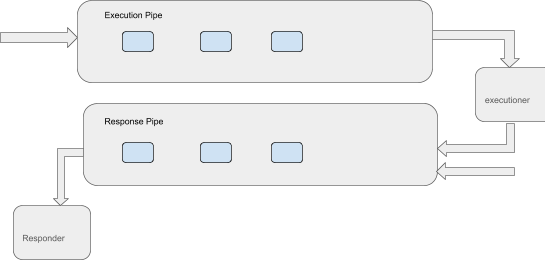
\includegraphics[scale=0.5, width=100mm]{poll}
    \centering
    \caption{Execution Pipe}
    \label{fig:poll}
\end{figure}

    \end{adjustwidth}

    \textbf{Execution Engine}\\
    \begin{adjustwidth}{1cm}{}
        It consists of two pipes (Execution and Response). A task is put into the execution pipe then
pulled by the executioner to be executed. If a problem occurs (failed to connect to the
database server) during execution, the executioner will then put the task back in the execution
pipe for another trail.\\
If the execution produces a result, like for example (GetCustomer), it will be put into the
response pipe to be sent back to the invoker of the Task and so on.\\
This helps when a problem led to make the services requests through API call unable to be
invoked. For example, failed to connect to the data source, so the solution is instead of
invoking them when requested through the API, which will lead to failure, we put them into
the Execution Queue and we know the rest.\\
Another big use is when the service requested through the API is not atomic or it’s atomic but
Time-consuming, in that case, the services can be put one by one into the execution pipe and
it will be taken care of. This will make the system more responsive.
    \end{adjustwidth}
        
        
    
    
\end{adjustwidth}

\section{The Modules}

The modules are interconnected with each other and often have jobs to that each will have a share in
like and they are integrated using the ERP.\\
The modules can be added separately to give users the customization and the choice of their business
needs without overwhelming them with unneeded modules.\\
Our modules including, but not limited to, as we are working on new modules
\begin{itemize}
    \item CRM
    \item Warehouse Management
    \item Accounting
    \item Manufacturing
\end{itemize}

\break
\subsection{CRM}
CRM (Customer Relationship Management) is a strategy to manage the relationships of the company.
It makes communicating with customers easier and improves marketing.
\begin{center}
    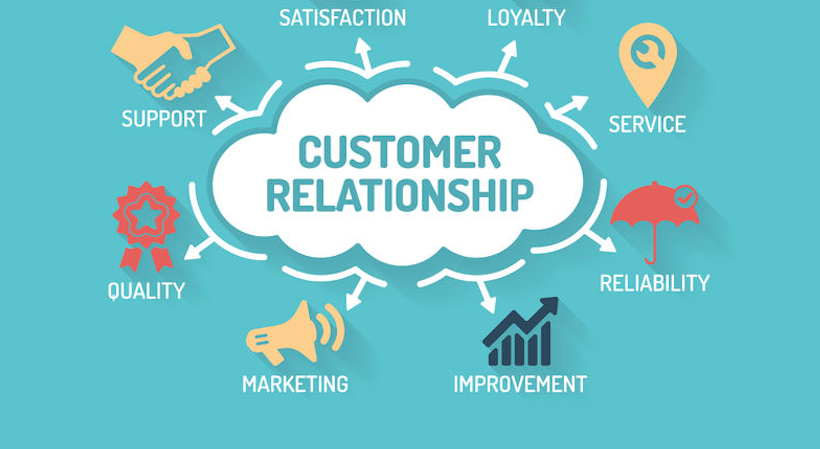
\includegraphics[width=\linewidth]{crm}
\end{center}

%\begin{figure}
%    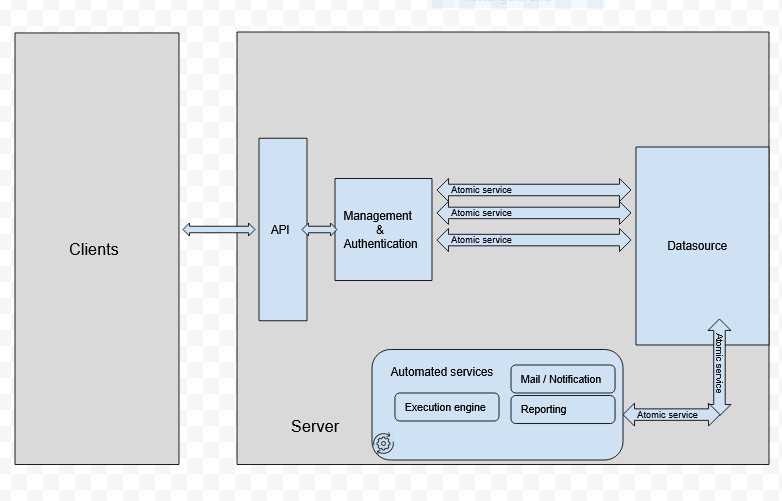
\includegraphics[width=\linewidth]{system_structure}
%    \caption{Test}
%    \label{fig:system_structure}
%\end{figure}
\subsubsection{Main features of CRM}
\begin{itemize}
    \item Customer Management
    \item Sales Management
    \item Reporting
\end{itemize}
\subsubsection{Customer Management}
We collect and manage customer information and their interests.
\begin{itemize}
    \item Qualified customers (Who have made orders)
    \item Non-Qualified customers (Who are considered to be the lead or target of the sales team)
\end{itemize}
Sales team communicates with non-qualified customers to make deals according to their interests of
products.\\
If the customer accepts the deal, an opportunity, that has some products of customer’s interests, is
created.
\subsubsection{Sales management}
We manage the sales through a pipeline of opportunities, each opportunity goes through 5 main stages
which are (New, Qualified, Proposition, Negotiation, and Won).\\
When an opportunity is created, it is in New stage, then a salesperson communicates with the
customer to make a deal with them. If the customer accepts the deal, the opportunity will be changed
to Qualified.\\\\
After that, a salesperson proposes some products that the customer has an interest in and negotiates
about their price. If the customer accepts to buy this product, the opportunity will be changed to Won
and will be created as an order in the system’s database.
\subsubsection{Reporting}
With CRM, salespeople and managers have access to dashboards where they can easily view
important opportunity KPIs, in the form of graphs, charts, and more. They can also export data and
create reports. This allows employees to analyze opportunities, and thus gain insights into sales and
marketing activities. You can also analyze lost/won opportunities to improve your conversion rates.
\newpage

%\begin{figure}
%    \centering
%    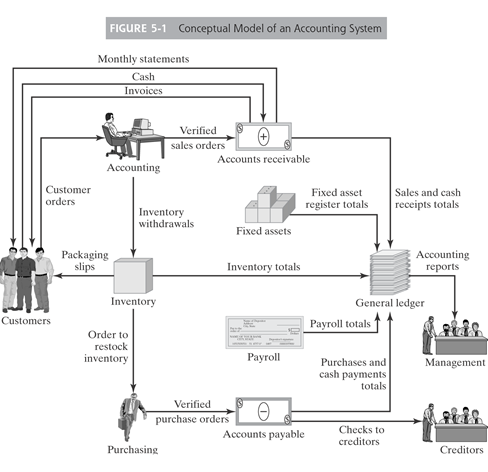
\includegraphics[width=\linewidth]{crm_workflow}
%   \caption{CRM Workflow}
%    \label{fig:crm_workflow}
%\end{figure}

\subsection{Warehouse management}
Warehouse management refers to the various processes related to maintaining and controlling a
business’ warehouse, such as the shipping, receiving, put-away and picking of goods. Warehouse
management is responsible for everything that happens in a warehouse, whether they own one
warehouse or several.\\\\
Managing inventory in warehouses with pen and paper can be inaccurate, slow and a lot of work,
that’s why it’s better to use a Warehouse management system.

\begin{center}
    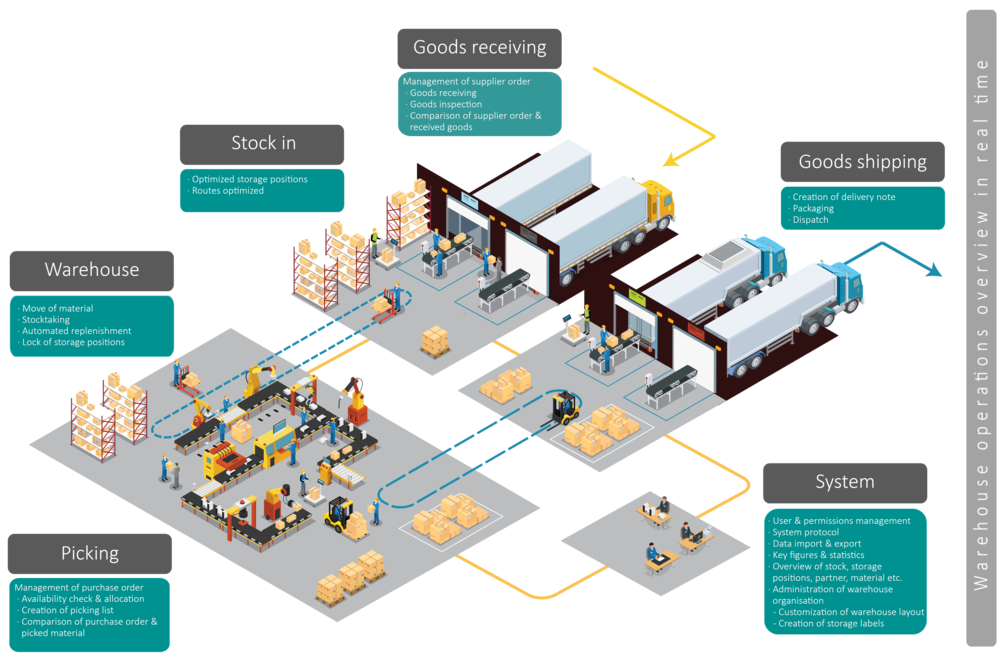
\includegraphics[width=\linewidth]{wms}
\end{center}

\subsubsection{Warehouse management system}
Warehouse management system (WMS) is a piece of software that controls, records and automates
various warehouse operations. The goal is to increase the overall productivity and efficiency of a
business’ warehousing operations.
\subsubsection{What about our implementation of WMS ?}
Our WMS can be used as a standalone system or can be integrated into The ERP. It supports multiple
inventories, keeps track of products’ moves, provides constant reports about orders delivery time, and
has many other features.
\subsubsection{Features}
Uses a database configured to support warehouse operations, containing details describing a
variety of standard warehouse elements including
\begin{itemize}
    \item Individual items that are handled and stored using weight, dimensions, automatic ID
    labels (bar codes, etc.), number of units in inventory, location in inventory, and
    whether it’s sold or purchased
    \item Warehouse storage location and size
    \item Orders that are handled using automatic order number, customer’s information,
    payment details, and time and date details (order being made, order ready for
    shipping, and order delivery to the customer)
    \item Ordered items with their quantities
    \item Supply requests with their time and date, suppliers’ information, and the number of
    units to be supplied
\end{itemize}
Is responsible for
\begin{itemize}
    \item providing Status of item quantity in terms of in stock, ordered, and ready for shipping
    quantities
    \item Handling Multiple warehouses
    \item Following up with each order throughout its stages from being made until it’s ready
    for shipping
    \item Keeping track of products going in and/or out of inventories
    \item Organizing - sequencing the orders to be picked
    \item Reporting, which helps analyze the performance of warehouse operations, and find
    areas to improve
    \item Asking for supply when an item is out of stock
    \item Sending notifications when an order is completed
\end{itemize}
\subsubsection{Benefits}
\begin{itemize}
    \item Track locations, transaction histories, and costing
    \item Speed up the process of getting products into and out of inventory by keeping records of the
    location of each product inside the inventory
    \item Organizing - sequencing the orders to be picked helps Minimize the need for dock staging
    space, by having orders arrive at the shipping dock in trailer load sequence
    \item Proper reporting mechanism of inventory helps the manufacturing department in planning
    their future production schedules accordingly
    \item It helps track the payments and flow of finances into your Accounts
\end{itemize}
\newpage

%\begin{figure}
%    \centering
%    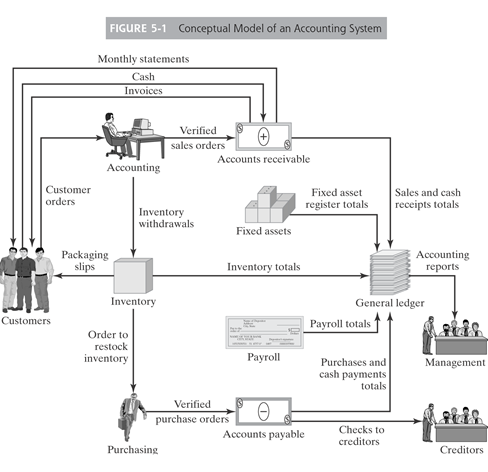
\includegraphics[width=\linewidth]{wms_workflow}
%   \caption{WMS Workflow}
%    \label{fig:wms_workflow}
%\end{figure}

\subsection{Accounting}
\begin{center}
    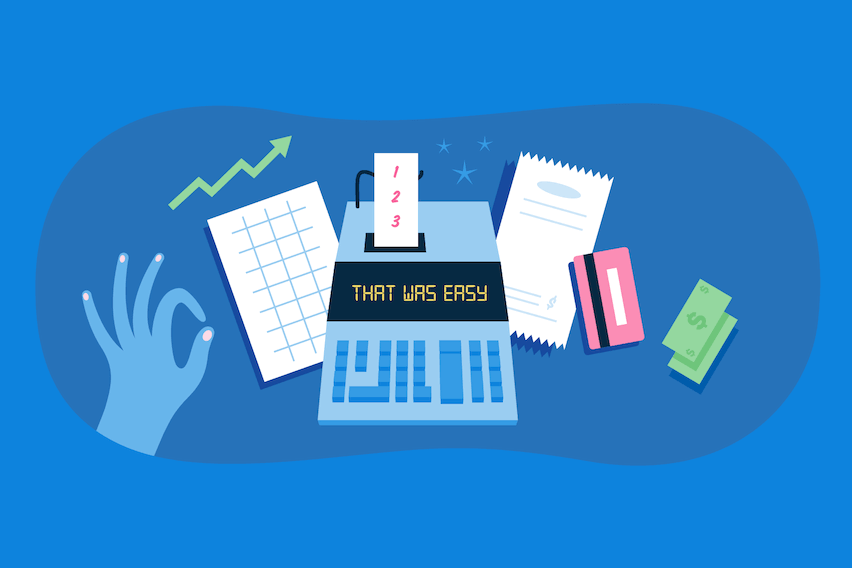
\includegraphics[width=\linewidth]{accounting}
\end{center}
\subsubsection{Why Accounting ?}
The financial module in ERP Systems provides financial functionality and analysis reports for balance
sheets, ledgers, and financial statements.\\\\
Financial module is essential for an organization. Other modules cannot function without it.
Successful implementation of financials is highly required for an organization in order to be trusted.
All these factors explain the fact that financial modules are taken up first.\\\\
The finance module of an ERP system has the following sub-systems.
\subsubsection{Accounting Subsystems}

\begin{adjustwidth}{2cm}{}
\textbf{Financial Accounting}
    \begin{adjustwidth}{1cm}{}
        The objective of a good Financial accounting system is to provide control and integration
of financial information that is essential to strategic decision making. The Financial
accounting module of an ERP System gives you the ability to track financial accounting
data within an international framework of multiple companies, currencies, and charts of
accounts.\\
    \end{adjustwidth}
\textbf{General Ledger}
    \begin{adjustwidth}{1cm}{}
        General Ledger is essential to both, the financial accounting system and strategic decision
making\\
    \end{adjustwidth}
\textbf{Accounts Receivables}
    \begin{adjustwidth}{1cm}{}
        The Accounts Receivable Modules helps in tracking all the invoices that are awaiting
payment from customers\\
    \end{adjustwidth}
\textbf{Account Payable}
    \begin{adjustwidth}{1cm}{}
        Accounts Payable Module (AP) — provides the functionality to enter, monitor, maintain,
and process for payment of invoices and credit notes that the organization received from its
vendors\\
    \end{adjustwidth}
\textbf{Asset Accounting}
    \begin{adjustwidth}{1cm}{}
        \begin{itemize}
            \item Fixed asset management like acquisition, depreciation, retirement, etc
            \item Legal consolidation
        \end{itemize}
        A Legal consolidation process is a financial process that allows showing the assets,
financial position, and income of a group as if the group were a single enterprise\\
    \end{adjustwidth}
\textbf{Controlling}
    \begin{adjustwidth}{1cm}{}
        Controlling enables the possibility to plan the financial parameters of the company and
offers both, proactive capabilities for early warning if they become negative and complex
analysis tools to identify factors of influence\\
    \end{adjustwidth}
\end{adjustwidth}
\subsubsection{Accounting Processes}
\begin{adjustwidth}{2cm}{}

    \textbf{Budgeting}
        \begin{adjustwidth}{1cm}{}
            Analysis of allocations, expenditures, revenues\\
        \end{adjustwidth}
    \textbf{Cash management}
        \begin{adjustwidth}{1cm}{}
            Cash flow analysis\\
            What-if analysis\\
        \end{adjustwidth}
    \textbf{Capital budgeting}
        \begin{adjustwidth}{1cm}{}
            Evaluation tools: NPV, IRR, pay-back period\\
        \end{adjustwidth}

\end{adjustwidth}
\subsubsection{Our Module Features}
\begin{itemize}
    \item Show Company Accounting data
    \begin{itemize}
        \item Show Sales (The products sold and how much the company earned)
        \item Show Bills (Show the bills that the company has to pay and how much money is it)
        \item Show Payments (Show the payments the company made, buying products materials
        or paid for bills)
        \item Show Company invoices (For the payments have been made, if there was any)
    \end{itemize}
    \item Show Customers Accounting Data
    \begin{itemize}
        \item Billing data (Show the bills that the customer has to pay for the company)
        \item Invoices data (Show the customer’s invoice for each payment for the order he has
        made)
    \end{itemize}
    \item Show Real-time data
    \begin{itemize}
        \item To show data as soon as it changes with no need to refresh the page
    \end{itemize}
    \item Reporting
    \begin{itemize}
        \item Reports about profits, losses, and balance sheets
    \end{itemize}
    
\end{itemize}

%\begin{figure}
%    \centering
%    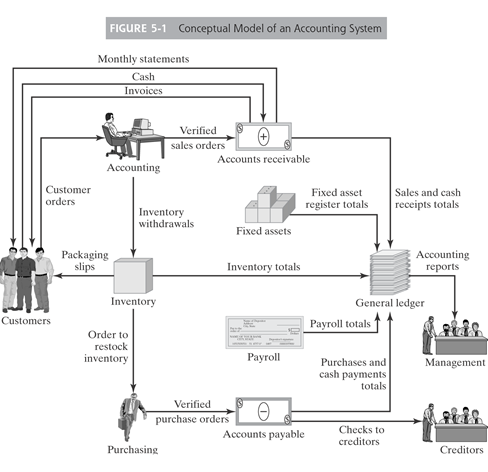
\includegraphics[width=\linewidth]{accounting_workflow}
%   \caption{Accounting Workflow}
%    \label{fig:accounting_workflow}
%\end{figure}

\break

\subsection{Manufacturing}
\begin{center}
    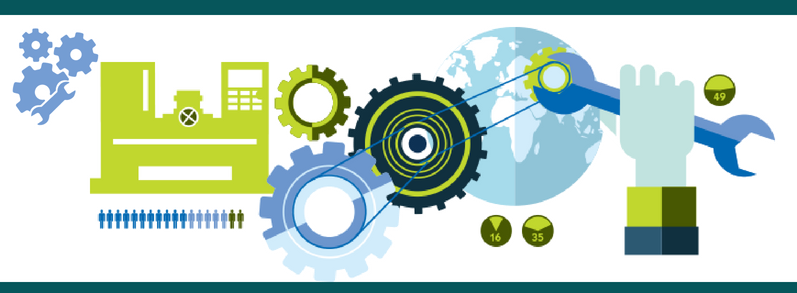
\includegraphics[width=\linewidth]{manufacturing}
\end{center}

In order to sustain in the stiff competitive market, manufacturing companies invest a lot of time
managing their diverse business functions rather than focusing on core business. This eventually leads
to less productivity and profitability in the business sector.\\
A manufacturing management software comes with an ample number of features that helps in
streamlining business operations, effectively transacting information across all business sectors,
ultimately focusing on enhancing the business workflows.\\
Manufacturing is the process by which raw materials are transformed into finished products.

\subsubsection{Manufacturing Module}
The role of ERP manufacturing module is to complete the inventory management by implementing
the operations specific to a streamlined manufacturing process. For a company, which handles a large
number of manufacturing products, they need to track every manufacturing order efficiently and
effectively.

\subsubsection{Our implementation of Manufacturing Module}
The Manufacturing Module in our system is independent and robust in handling the complexity of
Production, managing bills of materials, planning the manufacturing Orders, etc. Manufacturing
module is one of the basic applications in our system. Since the Manufacturing module is highly
integrated with Inventory Management, you can keep your inventory automatically updated with each
manufacturing process.\\
Our implementation of the manufacturing module helps businesses by dealing with the following
subjects
\subsubsection{Products}
Manufacturing module gives you the ability to add your manufacturing end products and determine a
bill of materials for each product by using a friendly user interface.
\subsubsection{Bill of materials}
Bill of Materials (BoM) is the basic building block of any manufacturing process. It is the list of raw
material needed to produce a product. So while creating a manufacturing order for a particular
product, one needs to select corresponding BoM. BoM will help the user to keep the inventory
updated during the manufacturing process.\\
BoM allows a flexible environment for custom builds without starting from scratch.
\subsubsection{Manage Production}
Once you have created and confirmed a Manufacturing order, you can start production. Our system
will list all the Manufacturing orders.\\
After making your order, our manufacturing system will place your orders in a list describing the
status of your order according to the inventory management system, starting date, and the current state
of your order (done, canceled, confirmed).
\subsubsection{Robust Inventory Tracking}
Manufacturing plants deal with raw material and finished goods inventory. Raw material management
is the process of keeping track of all appropriate material required to ensure that the business carries
on uninterrupted manufacturing processes. On the other hand, finished goods inventory includes
products that the manufacturing plant has produced, and they need to be managed to keep track of
how and when they would be transported to the warehouses or customers.\\
This is where many manufacturing modules experience challenges, as these two processes must be
synchronized to avoid inappropriate or insufficient production, which would bring customer
dissatisfaction, and cause losses to the business.\\
Keeping watch on these manually is quite impossible. For this, you need an ERP software that can
track complete inventory. The automated application would help reduce human errors and improve
inventory management like raw materials re-ordered needs or track the delivery dates of the finished
goods, etc., thus keeping your manufacturing running seamlessly.\\
From that context, our manufacturing system has a robust inventory tracking since you have placed
your order and in case of lacking raw materials, manufacturing module will change the status of your
order to waiting, until the raw materials are available. Our manufacturing module will track these
changes and update your order status.

\subsubsection{IOT Box}
IOT Box is one of the important features that our system offers, As it provides a way for the system to
communicate with hardware components directly. This will give the business even more managing
capabilities by integrating the hardware in the system to monitor the hardware and the process it does.\\
IOT box is a physical box that we offer that can be connected to our system directly and the box can
be then connected to the business hardware, like physical machines, to do its job.\\
The current IOT box is limited in features as it will send commands to the box that can in return send
them to the hardware we want to control. It works as a microcontroller that can be programmed from
the system to do its functions.\\
The IOT box is tended to have more capabilities and have different ports added to it to be used for
different activities.

%\begin{figure}
%    \centering
%    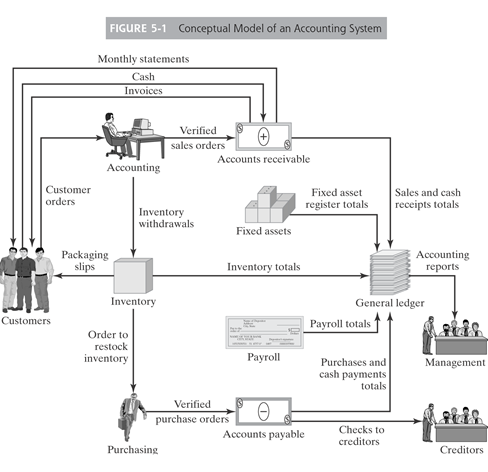
\includegraphics[width=\linewidth]{manufacturing_workflow}
%   \caption{Manufacturing Workflow}
%    \label{fig:manufacturing_workflow}
%\end{figure}

\break
\subsection{Product Manager}

\begin{center}
    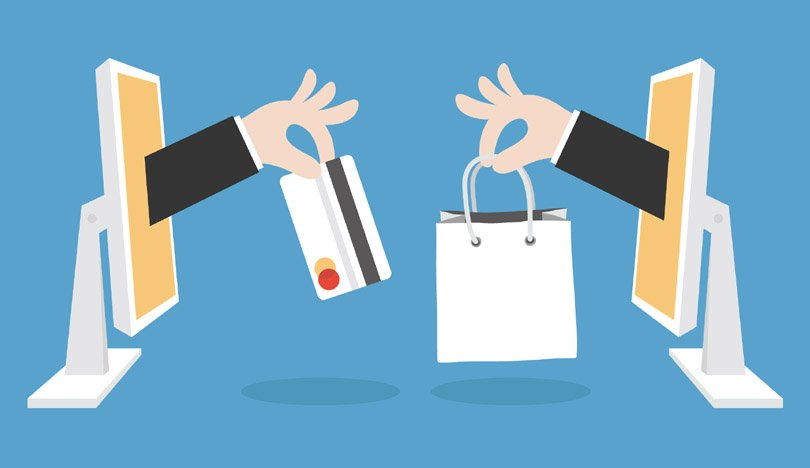
\includegraphics[width=\linewidth]{product}
\end{center}

Product manger do manage products

\chapter{System Access}

\section{The ERP}
We wanted to achieve, with The ERP, the ability for the users to be able to use the system from
anywhere to give the users more diversity of the places they can check the system from or achieve
tasks and also give the users the ability to determine what can be achieved and from where to satisfy
business rules and security.\\\\
To achieve this. The ERP comes with more than one plan, the first is to have the code for the program
and use it within the company.\\\\
To achieve the more diversity options, The ERP will be on the cloud for different businesses to use
and benefit from it, which allows users to access it from anywhere and also with a mobile app to have
a more concise view of the system.

\section{Mobile Application}
\subsection{ERP App Main Task}
The main task of the ERP app is to provide an easy way to monitor the modules of the ERP system
\subsection{Main Features}
\begin{itemize}
    \item Authenticate admins
    \item Authenticate users
    \item Rest API with the main ERP server
    \item Display all modules
    \item Display statistics of each module
\end{itemize}

\subsection{Application Screens}
\begin{itemize}
    \item \textbf{Authentication sign up screen}\\ Responsible for registering the full data needed of the customer or the admin of the
    module.
    \item \textbf{Authentication login screen}\\ Responsible for getting email and password from the user for authentication.
    Get the user type if admin or customer.
    \item \textbf{Modules Screen}\\ Displays all modules
    \item \textbf{CRM Screen}\\ Displays more information about the module and some statistics about the customers
    \item \textbf{Billing \& Accounting Screen}\\ Displays more information about the module and some statistics
    \item \textbf{Warehouse Management Screen}\\ Displays more information about the module and some statistics
    \item \textbf{Profile Screen}\\ Displays the current modules and some settings of the application

\end{itemize}

The ERP application is made with flutter which is Google’s mobile app SDK, complete with a
framework, widgets, and tools, that gives developers an easy way to build and deploy visually
attractive, fast mobile apps on both Android and iOS platforms.
